\documentclass[mathserif]{beamer}

\usepackage[utf8]{inputenc}    % enables use of utf8 characters in the input file
\usepackage[T1]{fontenc}       % enables proper output of unicode characters such that text can be copy-pasted from the pdf file
\usepackage{times}             % replaces Computer Modern font with something resembling Times
\usepackage{graphicx}          % enables including graphics
\usepackage{amsmath}           % ams math module
\usepackage{amssymb}           % ams math symbols
\usepackage{mathtools}         % fixes a few quirks with the ams packages

% functions
\DeclareMathOperator{\atan2}{atan2}
\DeclareMathOperator*{\argmin}{argmin}
\DeclareMathOperator*{\argmax}{argmax}

% braces
\newcommand{\xp}[1]{\left(#1\right)}   % parentheses
\newcommand{\xb}[1]{\left[#1\right]}   % brackets
\newcommand{\xc}[1]{\left\{#1\right\}} % curly braces
\newcommand{\xa}[1]{\left|#1\right|}   % absolute value
\newcommand{\xn}[1]{\left\|#1\right\|} % vector norm

% types
\newcommand{\function}[2]{#1 \rightarrow #2}
\newcommand{\R}[1]{\mathbb{R}^{#1}}
\newcommand{\RR}{\mathbb{R}}
\newcommand{\unit}{\xb{0,1}}

% complex terms
\newcommand{\apply}[2]{#1\!\xp{#2}}
\newcommand{\integral}[4]{\int_{#1}^{#2} #3 \; \mathrm{d}#4}
\newcommand{\powerset}[1]{\apply{\mathcal{P}}{#1}}

% continuity
\newcommand{\contp}[1]{\mathrm{C}^{#1}}
\newcommand{\contg}[1]{\mathrm{G}^{#1}}

% vectors
\newcommand{\vectorA}[1]{\begin{pmatrix}#1\end{pmatrix}}
\newcommand{\vectorB}[2]{\begin{pmatrix}#1\\\linebreak{}#2\end{pmatrix}}
\newcommand{\vectorC}[3]{\begin{pmatrix}#1\\\linebreak{}#2\\\linebreak{}#3\end{pmatrix}}
     % some math helper macros

\useoutertheme{miniframes}
\useinnertheme{default}
\usecolortheme{default}
\setbeamertemplate{navigation symbols}

\title{Optimal Fitting of Planar Curves to Prescribed Constraints}
\author{Julian Asamer, Julian Brunner}
\date{\today}

\begin{document}

	\begin{frame}
		\titlepage
	\end{frame}

	\section{Introduction}

		\begin{frame}
			\frametitle{Introduction}
			\begin{itemize}
				\item vector grapics are widely used
				\item 2D vector graphics primitives are curves
				\item design process of curves is very important
				\item designing curves with current tools can be frustrating
				% artist has a hard time to make the curve look the way he wants to
				% often unclear why
				% it's hard to communicate intentions
				\item research has been done in different direction with little impact
				\item our objective: improved curve design process
				% identify nature and cause of shortcomings in current curve design tools 
				% develop a better curve design tool
			\end{itemize}
		\end{frame}
		
	\section{Problem Analysis}
	
		\begin{frame}
			\frametitle{The Curve Design Process}
			\begin{itemize}
				\item obtain source curve
				% as real or mental image, obviously software-independent
				\item extract properties from the source curve 
				\item provide them to the software
				% strongly dependent on curve design tool - the software dictates which properties can be entered
				\item the software derives a curve
				% if the curve is not precisely specified, a fairment measure is used to derive the most likely result curve
				% iteration over steps 2-4 to adjust the curve until satisfactory alignment with the source curve is reached
			\end{itemize}
		\end{frame}
		
		\begin{frame}
			\frametitle{Usability Criteria for Curve Design Tools}
			\begin{itemize}
				% curve design tools can affect the design process by choosing specification language and fairness measure, and practical ability to derive curves from them
				\item description language := specification language + fairness measure
				\item specification language should be
				\begin{itemize}
					\item expressive
					% easy to handle for humans
					\item easy
					% allow efficient communication of intent
					\item efficient
				\end{itemize}
				\item fairness measure should ensure
				\begin{itemize}
					% capture intuitive notions of smoothness
					\item smoothness
					% select curves that are minimal in respect to the specification
					\item select minimal curves
				\end{itemize}
				\item ability to derive curves from descriptions
			\end{itemize}
		\end{frame}
		
	\section{Existing Curve Design Tools}
	
		\begin{frame}
			\frametitle{Bézier Splines}
			\begin{itemize}
				\item most commonly used
				\item edited by directly modifying coefficient points
				% the user can effectively specify start and end points as well as start and end velocities (which are proportional to the distance between the second and the first as well as the fourth and third point)
				% user supplies start and end point and velocity; fairness measure always chooses cubic Bézier spline.
				% which is uniquely specified
				\item most criteria fulfilled nicely
				% curvature continuity is not guaranteed
				% it is very hard to choose coefficient points in a way that results in curvature continuity.
				\item problems
				\begin{itemize}
					\item curvature continuity
					% curvature cannot be specified directly
					% constant/linearly changing curvature cannot be specified
					% circular arcs/spirals are very hard to specify
					\item problem: expressiveness of the specification language
				\end{itemize}
			\end{itemize}
		\end{frame}
		
		\begin{frame}
			\frametitle{Usability Analysis of Bézier Splines}
			\begin{centering}
				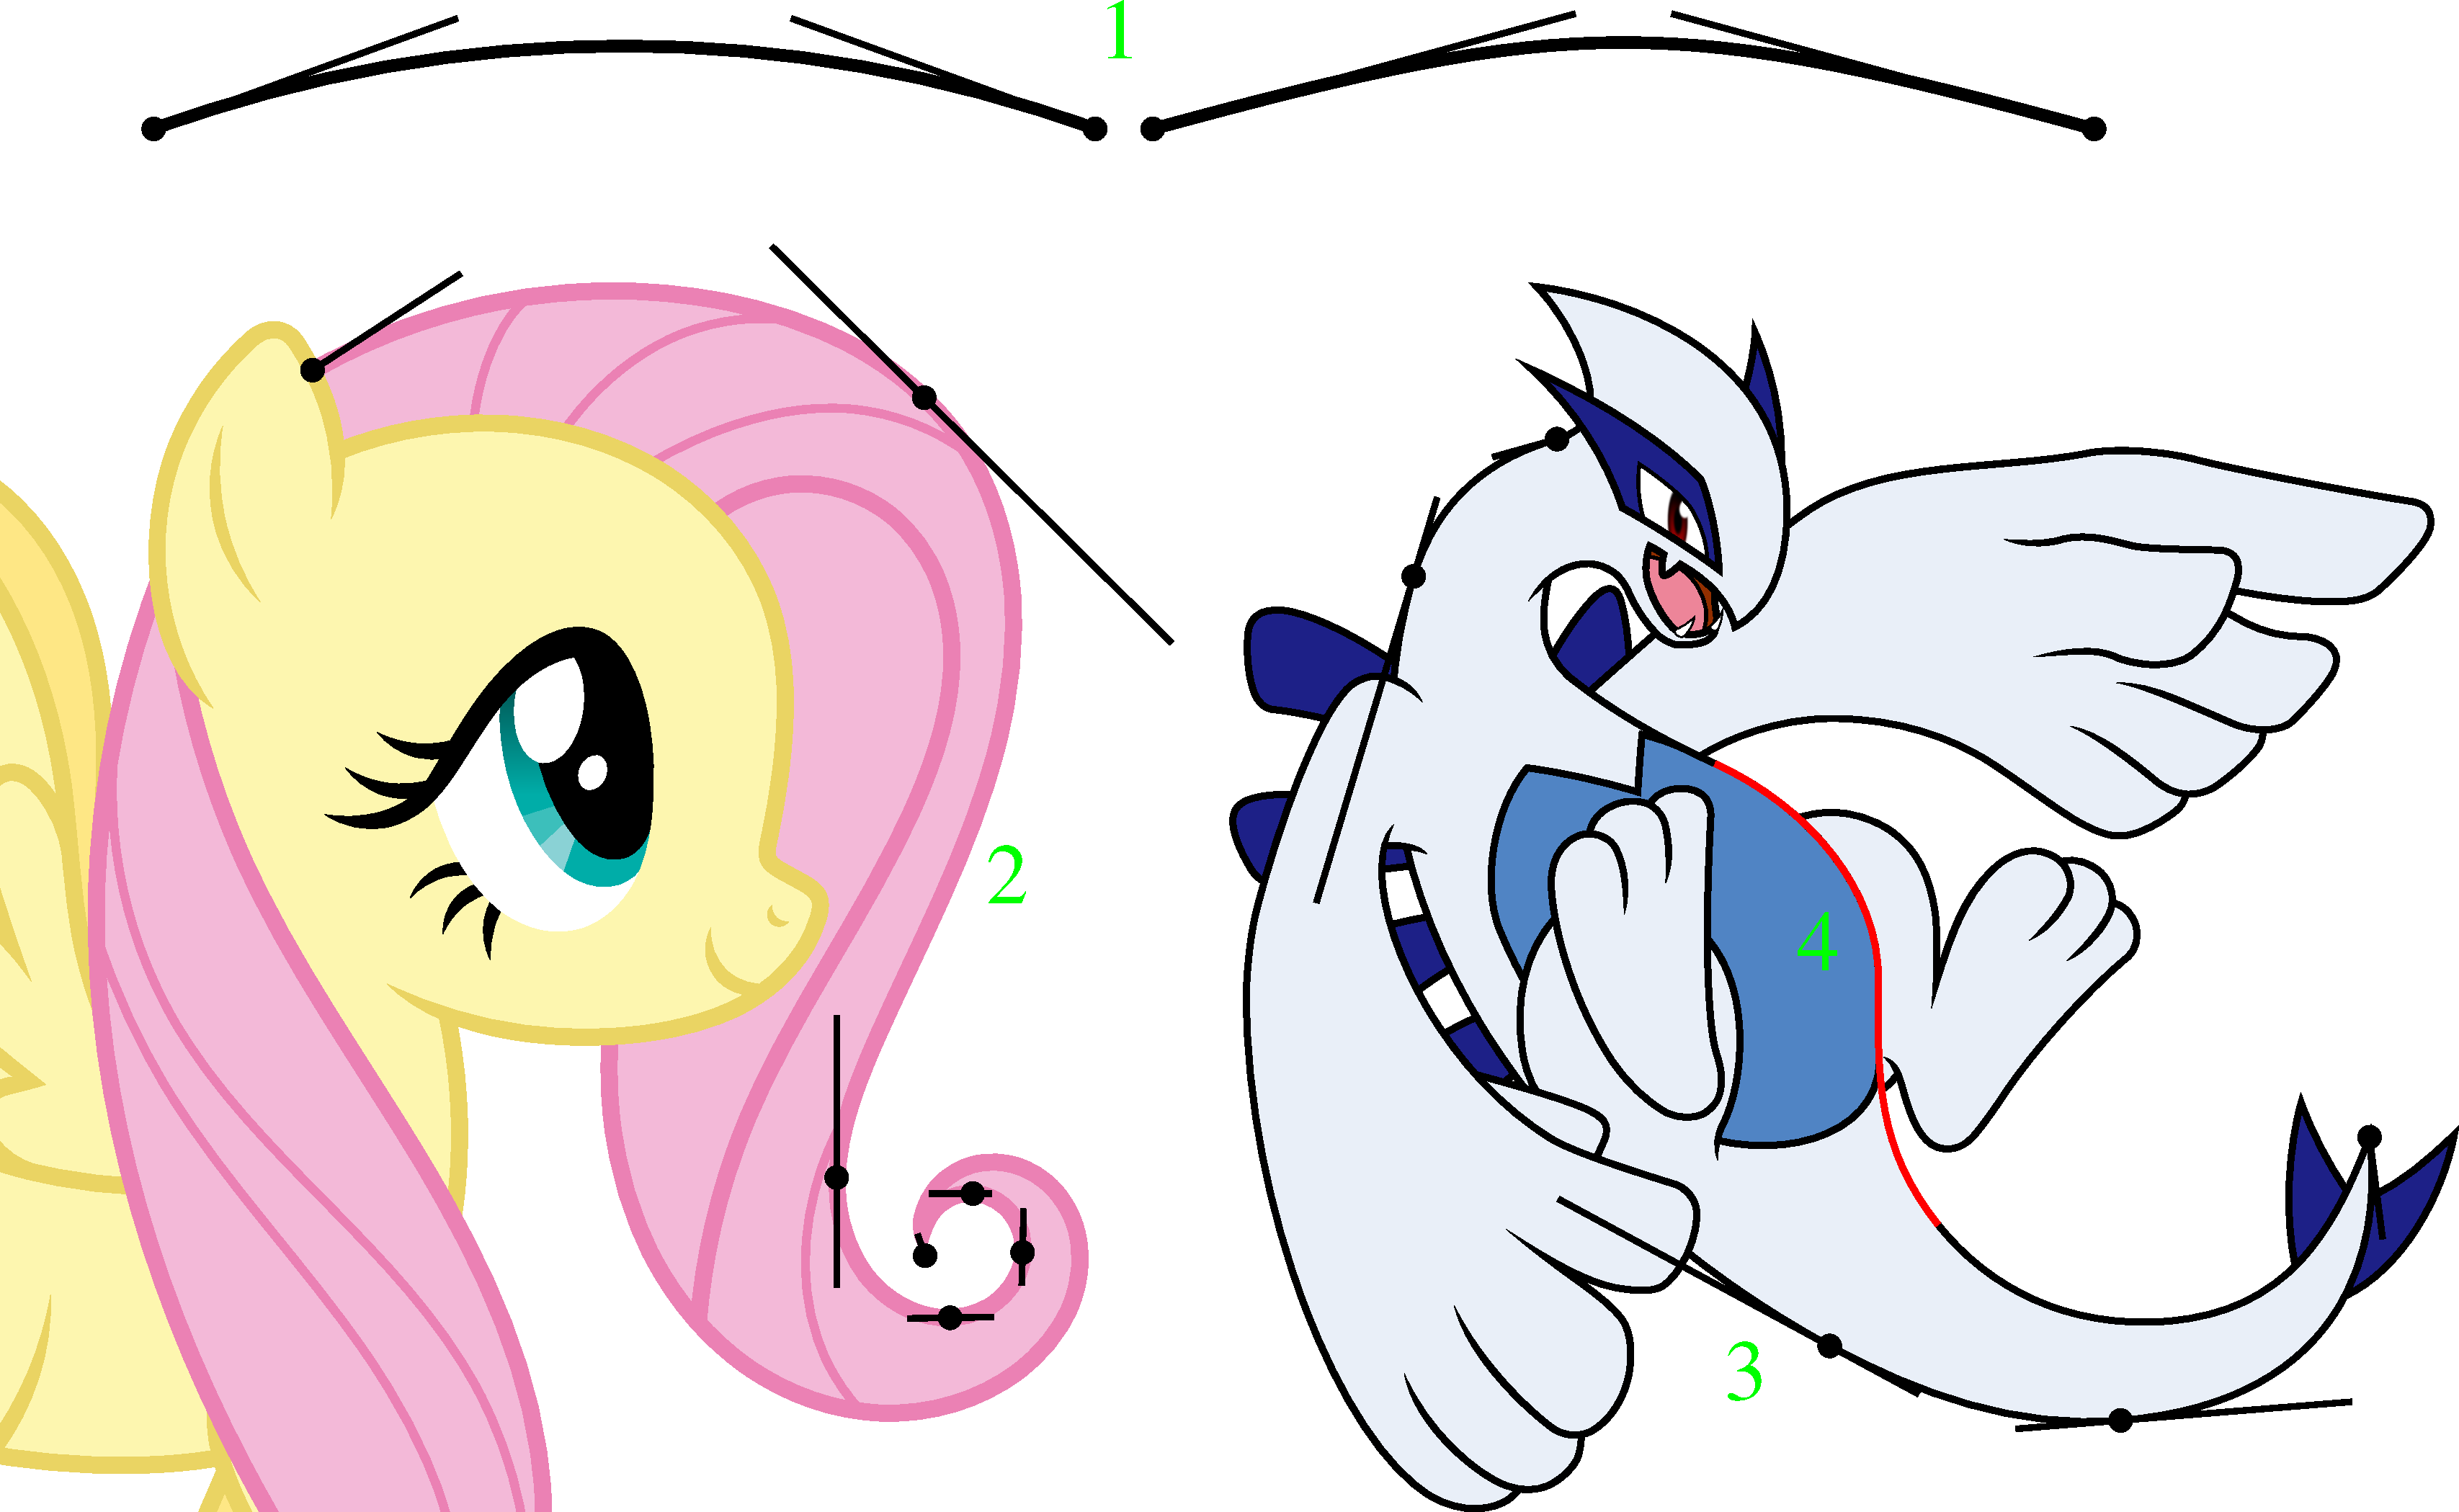
\includegraphics[width=\textwidth]{../resources/usability_bezier.pdf}
			\end{centering}
		\end{frame}
		
		\begin{frame}
			\frametitle{Spiro Splines}
			\begin{itemize}
				\item constructed from segments of the Euler spiral
				\item constructs interpolating splines
				\item can only specify points (no direction or curvature)
				\item guarantees curvature continuity
				\item problem: insufficient expressiveness of specification language
			\end{itemize}
		\end{frame}
		
		\begin{frame}
			\frametitle{Usability Analysis of Spiro Splines}
			\begin{centering}
				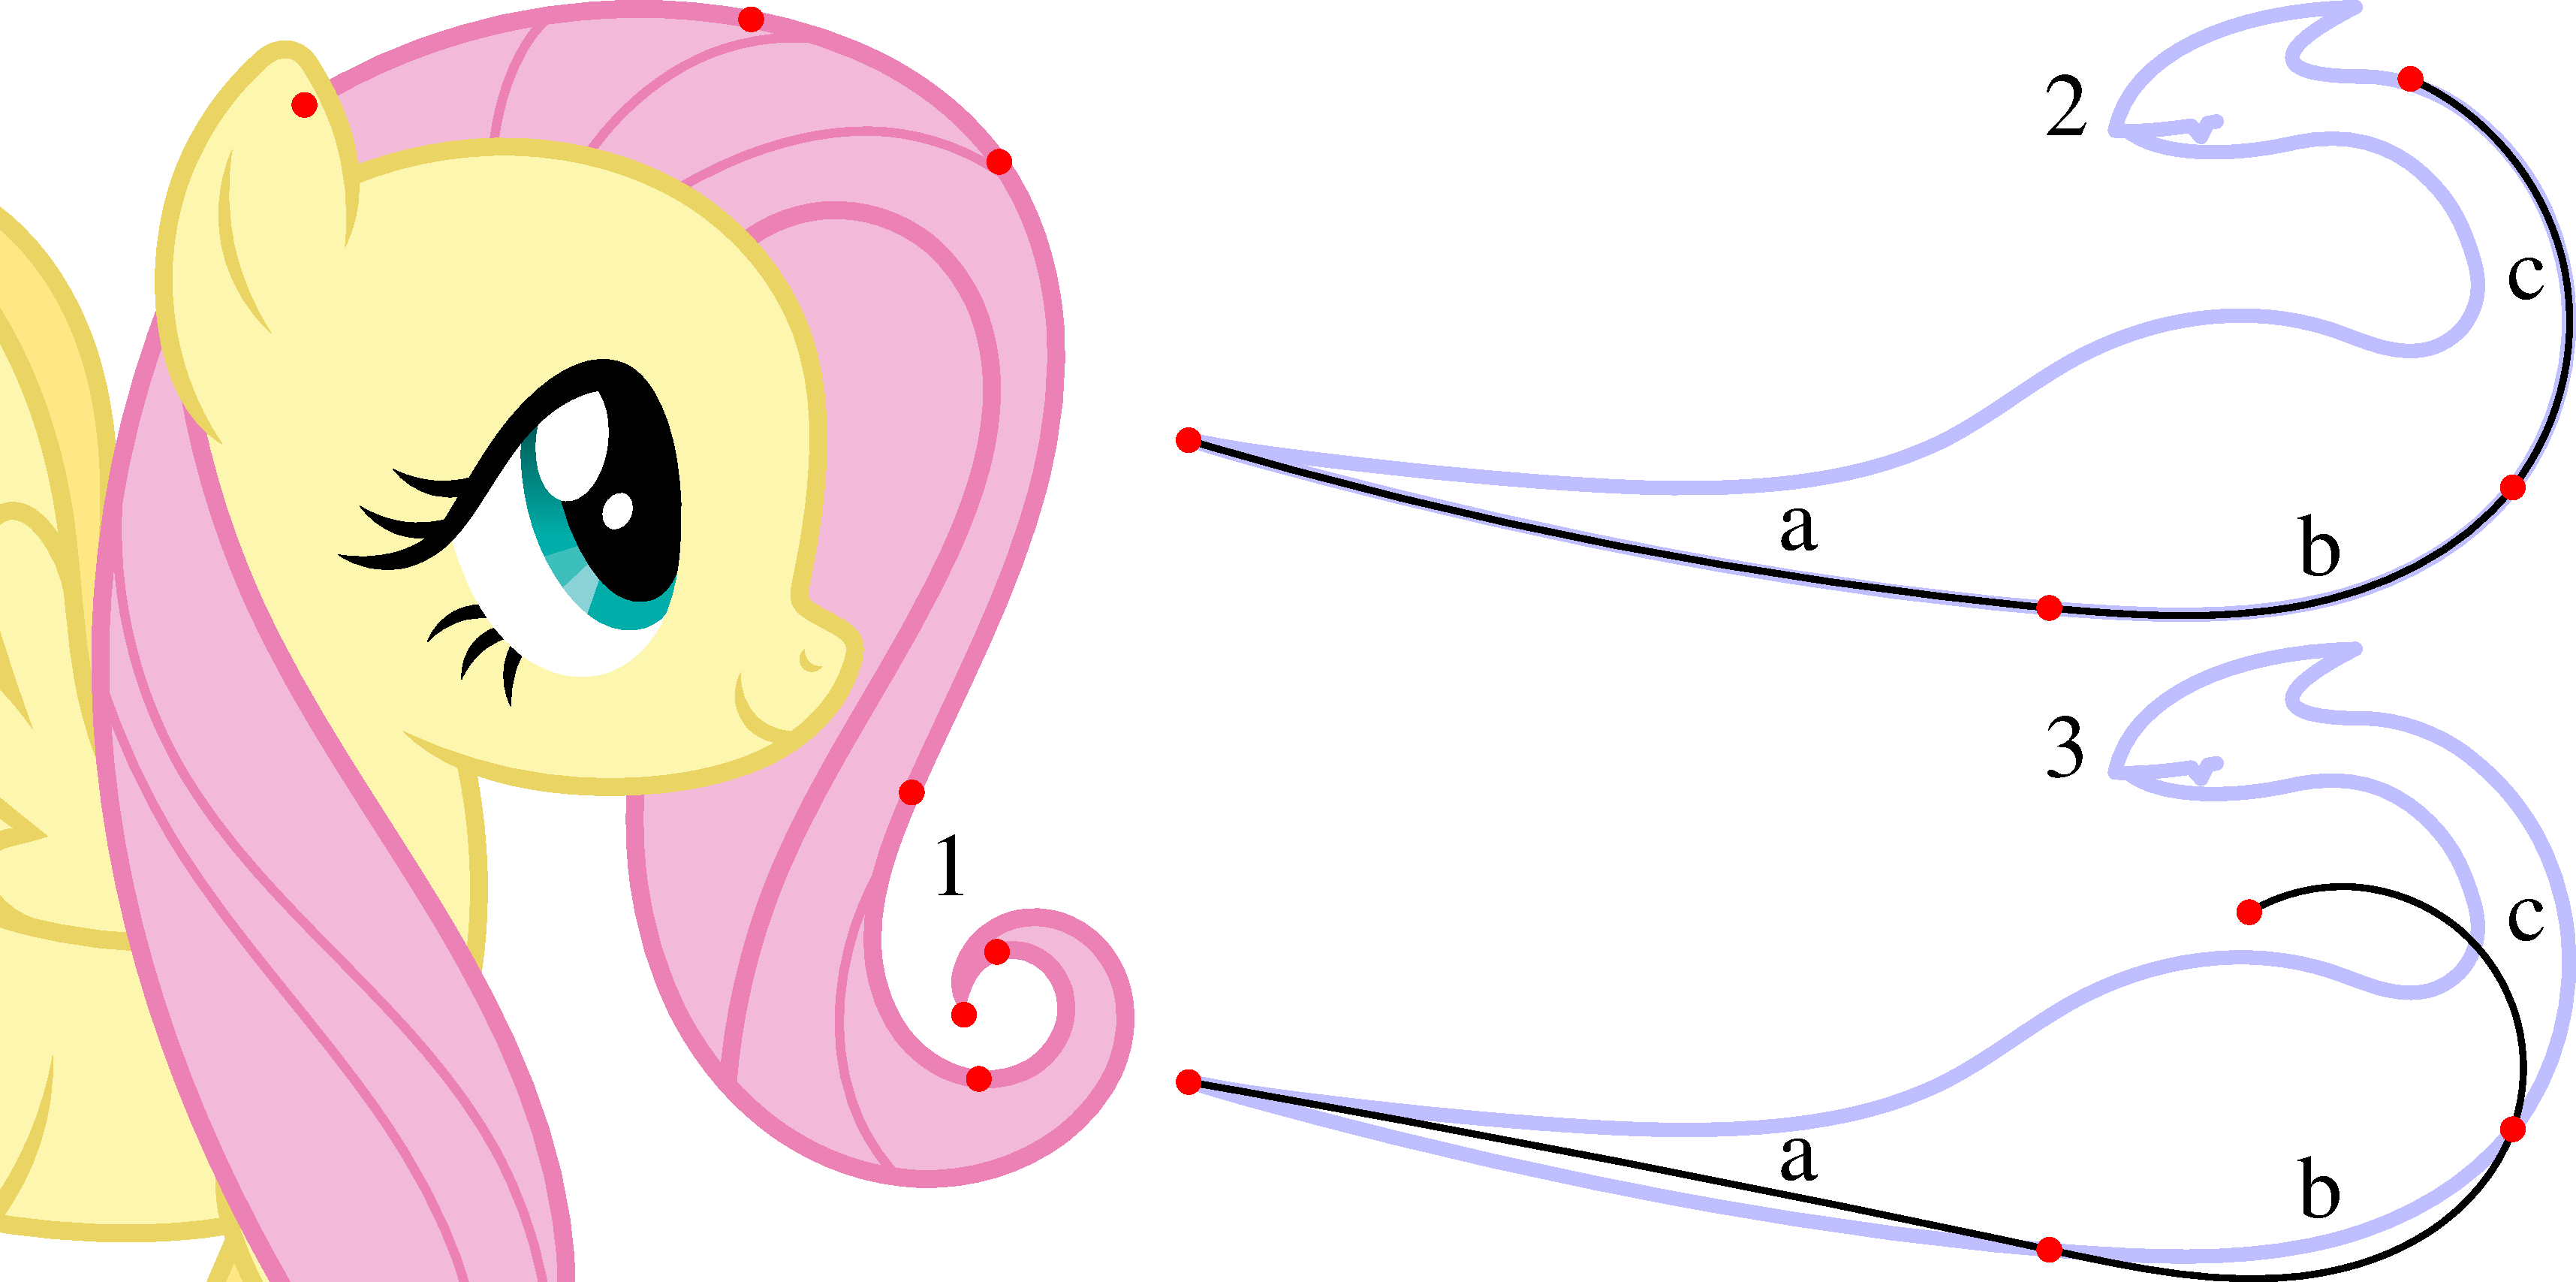
\includegraphics[width=\textwidth]{../resources/usability_spiro.pdf}
			\end{centering}
		\end{frame}
	
	\section{Proposed Solution}
	
		\begin{frame}
			\frametitle{Definitions}
			\begin{align*}
				\phi    & : \function{\unit}{\R{2}} && \text{point}\\
				\sigma  & : \function{\unit}{\RR}   && \text{speed}\\
				\lambda & : \function{\unit}{\RR}   && \text{covered arc length}\\
				\delta  & : \function{\unit}{\RR}   && \text{direction}\\
				\chi    & : \function{\unit}{\RR}   && \text{curvature}
			\end{align*}
		\end{frame}
		
		\begin{frame}
			\frametitle{Description-Based Curves}
			\begin{itemize}
				\item description language has huge effect on usability
				\item should not be based on low-level mathematical aspects % beziere
				\item do not impose limitations on specification language prematurely % spiro
				\item we need a good specification language and fairness measure
			\end{itemize}
		\end{frame}
	
		\begin{frame}
			\frametitle{Description-Based Curves}
			\begin{centering}
				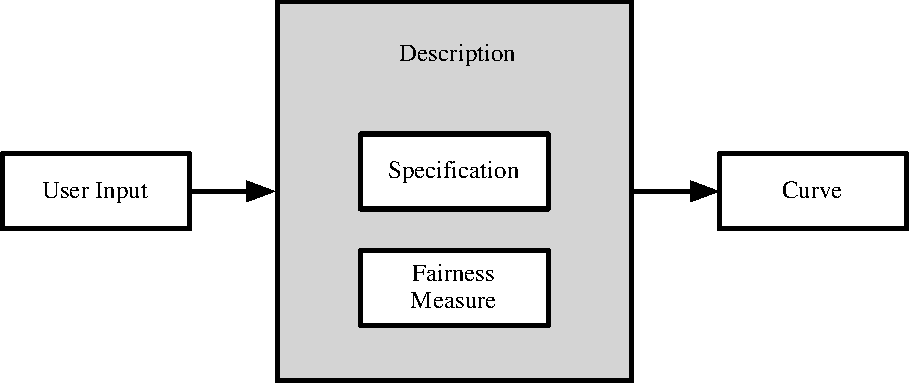
\includegraphics[width=\textwidth]{../resources/description-based_curves.pdf}
			\end{centering}
		\end{frame}
		
		\begin{frame}
			\frametitle{Specification Language}
			\begin{itemize}
				\item decoupled from underlying curve model
				\item allows specification of geometric properties
				\item point, direction, curvature
				\item any combination, any position
				\item positioning via fraction of arc length of curve
			\end{itemize}
		\end{frame}

		% TODO replace with ui screenshot
		\begin{frame}
			\frametitle{Specification Language}
			\begin{equation*}
				\begin{alignedat}{2}
					& \mathrm{Positions}          && = \unit\\
					& \mathrm{Points}             && = \R{2}\\
					& \mathrm{Directions}         && = \RR\\
					& \mathrm{Curvatures}         && = \RR\\
					& \mathrm{SpecificationItems} && = \mathrm{Positions} \times \left(\mathrm{Points} \cup \mathrm{Directions} \cup \mathrm{Curvatures}\right)\\
					& \mathrm{CurveLengths}       && = \RR\\
					& \mathrm{Specifications}     && = \powerset{\mathrm{SpecificationItems}} \times \mathrm{CurveLengths}
				\end{alignedat}
			\end{equation*}
		\end{frame}
		
		\begin{frame}
			\frametitle{Fairness Measure}
			\begin{itemize}
				\item chosen fairness measure: minimum variation curves
				\item captures intuitive notion of smoothness
			\end{itemize}
			 \begin{equation*}
				 \integral{0}{1}{\apply{\chi'}{t}^2}{t}
			 \end{equation*}
			 % TODO diagram comparing MVC and MEC
		\end{frame}
		
		\begin{frame}
			\frametitle{Curve Derivation}
			\begin{itemize}
				\item nonlinear optimization on polynomial splines % ie. segments described by polynomial curves
				\item nonlinear optimization: flexible, allows experimentation
				\item polynomial curves: simple yet flexible % through choice of degree
				\item polynomial splines: avoid polynomials of high degree
			\end{itemize}
		\end{frame}
		
		\begin{frame}
			\frametitle{Optimization Problem}
			\begin{itemize}
				\item expressed using:
				\begin{itemize}
					\item objective function \(f : \function{\R{n}}{\RR}\)
					\item constraint function \(g : \function{\R{n}}{\R{m}}\)
					\item constraint bounds \(g_l, g_u \in \R{m}\)
				\end{itemize} 
				\item tries to find an \(x^* \in \R{n}\) such that 
			\end{itemize}
			\begin{equation*}
				\begin{gathered}
					x^* = \argmin_{x \in \R{n}} \apply{f}{x}\\
					g_l \leq \apply{g}{x^*} \leq g_u
				\end{gathered}
			\end{equation*}
		\end{frame}
		
		
		\begin{frame}
			\frametitle{Finding Curves as Optimization Problem}

			Polynomials:
			\begin{equation*}
				\apply{\phi_i}{t} = \sum_j a_{i,j} \cdot t^j
			\end{equation*}

			Segmentation:
			\begin{centering}
				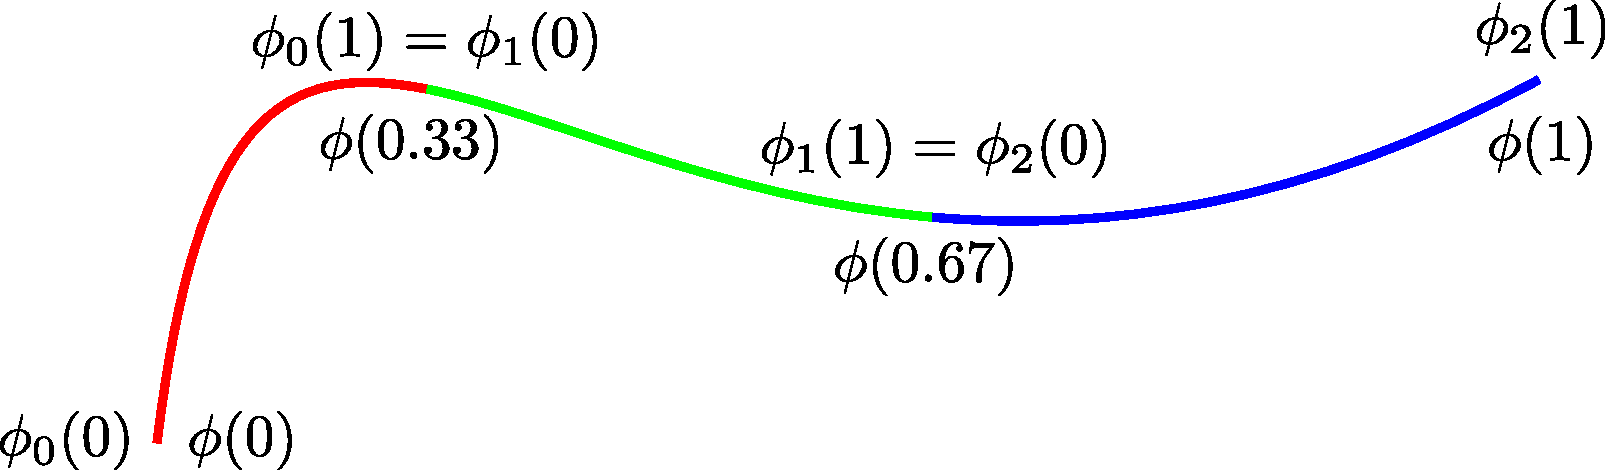
\includegraphics[width=\textwidth]{../resources/segmentation.pdf}
			\end{centering}

			\vspace{5mm}

			Optimization: Domain is coefficients \(a_{i,j}\)
		\end{frame}

		
		\begin{frame}
			\frametitle{Constant Speed}
			\begin{itemize}
				% specification's positions given as fraction of arc length; doesn't work very well in optimization process
				\item function mapping arc length to parameter value of curve needed
				% that function varies with coefficients, hence
				\item it is not possible to predict which segment a specification will end up on
				% fairness measure is integral over arc length of curve, hence
				\item fairness measure depends on mapping function
				\item solution: use following error term
			\end{itemize}
			
			\begin{equation*}
				\max_{t \in \unit} \xa{\apply{\sigma}{t} - \hat{\lambda}}
			\end{equation*}
			% cannot be fullfilled exactly by polynomials; hence no zero-error constraints. Implementations using an upper bound on errors and minimization goal were done; the latter yielded better results.
			
			\begin{itemize}
				\item covered arc length function is now linear
			\end{itemize}
			% because finding a maximum is not very suitable for smooth optimization
			\begin{equation*}
				\apply{\lambda}{t} \approx \hat{\lambda}t
			\end{equation*}
			% includes scaling in the beginning to make the error term scale invariant
		\end{frame}
		
		\begin{frame}
			\frametitle{Continuity Connections}
			\begin{itemize}
				\item whole spline has \(\contg{2}\) continuity
				\item each segment is smooth
				\item resulting spline is not
				\item continuity at the segment connection points needs to be ensured
				\item hence, we use constraints:
			\end{itemize}
			\begin{equation*}
				\begin{gathered}
					\apply{\phi_i}{1} - \apply{\phi_{i + 1}}{0}\\
					\apply{\phi'_i}{1} - \apply{\phi'_{i + 1}}{0}\\
					\apply{\phi''_i}{1} - \apply{\phi''_{i + 1}}{0}
				\end{gathered}
			\end{equation*}
			
			(\(\phi_i\) refers to the points of the i-th segment)
		\end{frame}
		
		\begin{frame}
			\frametitle{Fairness Error}
			\begin{equation*}
				\hat{\lambda}^2\integral{0}{1}{\apply{\chi'}{t}^2}{t}
			\end{equation*}
			\begin{itemize}
				\item can be arbitrarily large
				\item hence, it is a minimization goal
				\item factor \(\hat{\lambda}^2\) for scale invariance
				% enables static weighting of minimization goals
			\end{itemize}
		\end{frame}
		
		\begin{frame}
			\frametitle{Summary}
			\begin{itemize}
				\item construct optimization problem from error terms and constraints
				\item compute coefficients with solver
				\item build result curve from coefficients
			\end{itemize}
		\end{frame}
		
	\section{Implementation}
	
		\begin{frame}
			\frametitle{Architecture}
			\begin{itemize}
				\item programming language: C\#
				\begin{itemize}
					% familiar, high level
					\item platform independent
					\item interfaces with native code
					\item UI frameworks available
				\end{itemize}
				\item libraries
				\begin{itemize}
					\item IPopt: numeric nonlinear optimization
					\item CasADi: automatic differentiation of terms
					\item GTK\#: UI library
				\end{itemize}
			\end{itemize}
		\end{frame}
		
		\begin{frame}
			\frametitle{Subsystems}
			\begin{itemize}
				\item Kurve: UI prototype
				\item Kurve.Curves: optimization of curves
				\item Wrappers.Casadi and Wrappers.Casadi.Native: APIs for CasADi and IPopt
			\end{itemize}
		\end{frame}
		
		\begin{frame}
			\frametitle{Optimization Steps}
			\begin{itemize}
				\item segments
				\item optimization problem
				\item substitutions
				\item solver
				\item position
			\end{itemize}
			% diagram for dependencies
		\end{frame}
		
		% topics of the demo
		%
		% 1. explain features
		% 2. example mane fluttershy: specifying curvature is awesome. compare with beziere
		% 3. circle arcs via arc length (fluttershy chin/mouth/ear)
		% 4. maybe example for why fixed length might be undesirable
		% 5. euler spiral (we're doing it LIVE!)
		% 6. fairness: demonstrate with S-curve
		% 7. many local potentially shitty optima, can be fixed by stretching/dragging etc.
		% 8. Problem: slow
		% 9. May converge slowly or not at all
		% 10. Pathological local minima
		% 
		
		\begin{frame}
			\frametitle{Demo}
		\end{frame}
		
		\begin{frame}
			\frametitle{Conclusion}
			\begin{itemize}
				\item it works
				\item we are awesome
				\item `The most promising research in curve design tools in decades' - Albert Einstein
				\item future work
				\begin{itemize}
					\item test with users
					\item integrate into Incscape
				\end{itemize}
			\end{itemize}
		\end{frame}
\end{document}
